\documentclass[11pt]{article}
%\usepackage{ngerman}
\usepackage[english]{babel}
\usepackage{amsmath,amssymb,amstext}
\usepackage{graphicx}
\usepackage{parskip}
\usepackage{float}
\usepackage{tabularx}
\usepackage{amsmath}
\usepackage{placeins}
\usepackage{esint}
%\usepackage{subtextbf}
\usepackage{pdfpages}
\usepackage{url}
%\usepackage{cite}
\usepackage{array}
\usepackage{multirow}
\usepackage{hyperref}
\usepackage[style=numeric, backend=bibtex]{biblatex}
\usepackage{todonotes}
\usepackage{subcaption}
\usepackage{multirow}
\usepackage{upgreek}
\usepackage{circuitikz}





\addbibresource{references/references.bib}
\setlength{\textwidth}{15 true cm}
\setlength{\textheight}{22 true cm}
\oddsidemargin  0.5 cm
\evensidemargin 0.5 cm
\topmargin      0 cm

\renewcommand{\textfraction}{.2}
\renewcommand{\floatpagefraction}{.8}

\begin{document}
%\frontmatter
\pagenumbering{roman}

% Include titlepage
\begin{titlepage}	
	{\sffamily		
		\begin{center}			
			\includegraphics[width=30mm]{content/00_introduction/img/TU_Graz_Logo.png}
			
			\vfill\vfill\vfill
			\vfill\vfill\vfill
			
			{Simon Prato}
			% Author with existing titles
			
			\vfill\vfill\vfill
			
			{\LARGE\bfseries{Numerical Investigation of TEM Cells and Antenna Coupling}}
			% Title of the thesis			
			
			\vfill\vfill\vfill
			\vfill\vfill\vfill			
			
			{\bfseries\large{Master Thesis}}
			
			{Studies: {Electrical Engineering}}
						
			\vfill\vfill\vfill			
			
			submitted to
			
			\vfill
			
			{\bfseries\large{Technical University of Graz}}			
			
			\vfill\vfill\vfill			
			
			Supervisor
			
			{Dr. Thomas Bauernfeind}
			
			\vfill
			
			\vfill
			
			\includegraphics[width=30mm]{content/00_introduction/img/igte_logo.png}
			
			%% OPTIONAL: second supervisor/name of the faculty, etc.
					
			\vfill\vfill\vfill
					
			{Graz}, {August}~{2024}
			
		\end{center}
	}%% end sffamily
\end{titlepage}

\newpage

% Kurzfassung
\iftrue
\cleardoublepage
\setcounter{page}{2}
\vspace*{2.2 cm}
{\Large
\noindent
{\bf Abstract}} \\
\vspace*{0.3 cm}

\noindent

% Abstract
\cleardoublepage
\fi

\selectlanguage{english}
\listoftodos
% Inhaltsverzeichnis
	\tableofcontents  

% Tabellenverzeichnis
% optional
\newpage
	\listoffigures 

% Abbildungsverzeichnis
% optinal
\newpage
	\listoftables
	
\cleardoublepage

%\mainmatter
\pagestyle{headings}
\pagenumbering{arabic}

\section{Introduction}

\section{Theoretical Basics}

Magnetic and electric dipoles are an effective approach for modeling the radiation of electrically small antennas. They are defined as antennas with dimensions much less than one-tenth of the wavelength ($l\ll\lambda$)\cite[p. 151]{Balanis_1997}. By calculating the respective dipole moments, the coupling between antennas and TEM cells can be numerically estimated. This section provides a brief introduction to the underlying theory of this concept.

\subsection{Electric Dipoles}

An electric dipole is described as two tiny charged metal spheres or two capacitor-plates, which are connected with a linear wire of length $d$ and diameter $a$ \cite[p. 467]{Griffiths_2024}, \cite[p. 151]{Balanis_1997}. The charges move and accelerate along the wire, creating radiation. In case of an ideal, infinitesimal dipole, the wire is very thin ($a\ll \lambda$) and very small ($d \ll \lambda$) compared to the wavelength $\lambda$ \cite[p. 151]{Balanis_1997}, \cite[p. 468]{Griffiths_2024}. For an antenna to be accurately modeled as an infinitesimal electric dipole, its length usually must be smaller than a fiftieth of the wavelength ($d < \lambda/50$) \cite[p. 156]{Balanis_1997}. They are not very practical, but serve as a basic building block for more complex geometries. The current is spatially uniform throughout the wire.

Wires that are too long to be modeled as an infinitesimal dipole, but short enough to be considered electrically small ($\lambda / 50 < l \leq \lambda/10$), are classified as short physical dipoles \cite[pp. 162-163]{Balanis_1997}. They are a more accurate and useful representation of a linear wire antenna, and investigated further. In the remainder of this thesis, the term electric dipole refers specifically to short physical electric dipoles. Furthermore, time variation according to $\mathrm{e}^{-j\omega t}$ is assumed and therefore omitted.

A current $I_0$ is fed into the short, center-fed, linear antenna shown in \autoref{fig:electric_dipole}. The current along the antenna arms $I(z)$ linearly drops to zero \cite[p. 412]{Jackson}, as visualized in \autoref{fig:electricdipolecurrent}. Mathematically, it is described by, 

\begin{equation}
    I(z)= I_0\left( 1-\frac{2|z|}{d} \right).
    \label{eqn:current_dipole}
\end{equation}


\begin{figure}[h]
    \centering
    \includegraphics[width=0.5\linewidth]{content/10_theory/img/electric_dipole_drawing.png}
    \caption{Geometrical arrangement of a linear center-fed wire antenna.}
    \label{fig:electric_dipole}
\end{figure}

Charge accumulates along the antenna's arms. It is expressed as a charge per unit length $\rho'$ due to the thin wire. It is derived by the continuity equation,

\begin{equation}
    \rho' = \pm\frac{\mathrm{d}}{\mathrm{d}z}j\frac{ I(z)}{\omega} = \pm j\frac{2  I_0}{\omega d}.
    \label{eqn:charge_distribution_dipole}
\end{equation}

$\rho'$ is uniformly distributed along each antenna arm \cite[p. 412]{Jackson}.




An important metric is the electric dipole moment $\mathbf{p}$. It is defined as the product of charge density $\rho$ along the antenna and their source point $\mathbf{x'}$ \cite[p.410]{Jackson}, and generally expressed as 

\begin{equation}
	\mathbf{p} = \iiint_V\mathbf{x'} \rho (\mathbf{x'})\mathrm{d}\mathbf{x'}.
	\label{eqn:elec_dipole_mom}
\end{equation}

The vector $\mathbf{x}=\mathbf{\hat{a}}_x x + \mathbf{\hat{a}}_y y + \mathbf{\hat{a}}_z z$ represents the observation point coordinates, while $\mathbf{x'}=\mathbf{\hat{a}}_x x' + \mathbf{\hat{a}}_y y' + \mathbf{\hat{a}}_z z'$ represents the source point coordinates. The vectors $\mathbf{\hat{a}}_x$, $\mathbf{\hat{a}}_y$, and $\mathbf{\hat{a}}_z$ are unit vectors along the x-, y-, and z-directions, respectively. The integration is performed over the volume $V$ of the antenna.

Knowing the charge distribution $\rho'$ enables the calculation of the electric dipole moment $\mathbf{p}$ through \autoref{eqn:elec_dipole_mom}. This results in, 

\begin{equation}
    \mathbf{p}=\int_{-\frac{d}{2}}^{\frac{d}{2}}z\rho'(z)\,\mathrm{d}z\cdot\mathbf{\hat{a}}_z = j\frac{I_0d}{2\omega}\cdot\mathbf{\hat{a}}_z.
    \label{eqn:dipole_mom_example}
\end{equation}

The electric dipole moment $\mathbf{p}$ is parallel to the antenna's arms and points in the z-direction \cite[p. 412]{Jackson}, \cite[p. 155]{Griffiths_2024}. Next, the vector potential $\mathbf{A}$ is determined. It is generally defined as  \cites[p. 152]{Balanis_1997}[p. 410]{Jackson},
 
\begin{equation}
    \mathbf{A}(\mathbf{x})=\frac{\mu}{4\pi}\frac{\mathrm{e}^{-jkr}}{r}\iiint_V \mathbf{J}(\mathbf{x'})\mathrm{d}\mathbf{x'}.
    \label{eqn:vector_pot}
\end{equation}


The variable $r$ is the distance from any source point to the observation point $\left| \mathbf{x}-\mathbf{x'} \right|$. The permeability is described by $\mu$ and the term $\mathrm{e}^{jkr}$ the propagation of the wave, where $k=2\pi/\lambda$ is the propagation factor, or often called wavenumber \cite[p. 704]{Balanis_1997}. $\mathbf{J}$ is the current density in the source region. The calculations of $\mathbf{A}$ simplify to \cite[p. 410]{Jackson},

\begin{equation}
    \mathbf{A} (\mathbf{x})=-j\frac{\mathrm{\mu\omega}}{4\pi}\mathbf{p}\frac{\mathrm{e}^{-jkr}}{r}
    \label{eqn:vector_pot_elec_dipole}
\end{equation}
%Should the calculation of fields even be included? I don't need them for research. But the Field equations are important for explaining the frequency behavior of the electric dipole moment. This can be done by the radiation resistance in \autoref{eqn:elec_rad_res}. In our example, the radiation power depends on the frequency squared ($\mathbf{p}$\textasciitilde

\begin{figure}[t]
	\centering
	\includegraphics[width=0.3\linewidth]{content/10_theory/img/electric_dipole_current}
	\caption{Current distribution across linear wire antenna. It has a maximum at the feedpoint, and drops to zero at points $d/2$ and $-d/2$.}
	\label{fig:electricdipolecurrent}
\end{figure}


Any other field quantities can be derived out of the vector potential $\mathbf{A}$, such as the electric field intensity $\mathbf{E}$ and magnetic field intensity $\mathbf{H}$. This is achieved in a simpler way, when first transforming the Cartesian components of $\mathbf{A}$ into spherical ones, as demonstrated by \cite[p. 153]{Balanis_1997},

\begin{equation}
	\begin{bmatrix}
		A_r  \\
		A_\theta \\
		A_\phi
	\end{bmatrix} = 	
	\begin{bmatrix}
	\sin \theta \cos \phi & \sin \theta \sin \phi & \cos \theta\\
	\cos \theta \cos \phi &  \cos \theta \sin \phi & - \sin\theta\\
	- \sin\phi  & \cos\phi  & 0
	\end{bmatrix}
		\begin{bmatrix}
		A_x  \\
		A_y \\
		A_z
	\end{bmatrix}
\end{equation}

$\mathbf{E}$ and $\mathbf{H}$ are then expressed by \cite[p. 153]{Balanis_1997},

\begin{subequations}\label{eqn:elec_and_mag_field_dipole}
    \begin{equation}
    \mathbf{H} =\frac{1}{\mu r} \left[ \frac{\partial}{\partial r} (r A_{\theta}) - \frac{\partial A_{r}}{\partial \theta} \right]  \mathbf{\hat{\mathbf{a}}_\phi},
    \end{equation}\label{eqn:h_dipole}
    
    \begin{equation}
    \mathbf{E}=-j\omega\mathbf{A}-j\frac{1}{\omega\mu\epsilon}\nabla\left(\nabla\cdot\mathbf{A}\right).
    \end{equation}\label{eqn:e_dipole}
    
\end{subequations}

Substituting $\mathbf{A}$ into \autoref{eqn:h_dipole} and \autoref{eqn:e_dipole} reduces them to 

\begin{subequations}
	\begin{equation}
		H_r=H_\theta=0,
	\end{equation}
	\begin{equation}
		H_\phi = j\frac{k I_0 l \sin\theta}{4\pi r}\left[1 + \frac{1}{jkr}\right]\mathrm{e}^{-jkr},
	\end{equation}
\end{subequations}

and,

\begin{subequations}
	\begin{equation}
		E_r = \eta \frac{I_0 l \cos \theta}{2\pi r^2}\left[ 1 + \frac{1}{jkr} \right] \mathrm{e}^{-jkr},
	\end{equation}
	\begin{equation}
		E_\theta = j\eta \frac{kI_0 l \sin \theta }{4\pi r}\left[ 1 + \frac{1}{jkr} - \frac{1}{(kr)^2} \right] \mathrm{e}^{-jkr},
	\end{equation}
	\begin{equation}
		E_\phi = 0.
	\end{equation}
\end{subequations}


The total radiated power of the antenna is obtained by integrating the complex Poynting vector $\mathbf{W}$ over a closed surface surrounding the antenna \cite[p. 154]{Balanis_1997}. The real part of the total radiated power provides information about energy transferred by radiation, while the imaginary part about the antenna's reactive behavior. $\mathbf{W}$ is defined by 

\begin{equation}
	\mathbf{W}=\frac{1}{2}\left(\mathbf{E}\times\mathbf{H}^*\right) .
\end{equation}

The real power transfer is derived through the time-averaged Poynting vector $\mathbf{W}_\mathrm{av}$ \cite[p. 160]{Balanis_1997}, which is calculated by

\begin{equation}
    \mathbf{W}_\mathrm{av} = \frac{1}{2} \, \Re \{ \mathbf{E} \times \mathbf{H}^* \}.
    \label{eqn:time_averaged_poynting}
\end{equation}

By integrating the time-averaged real Poynting vector $ \mathbf{W}_\mathrm{av} $ over a closed surface, the radiated power $P_{\mathrm{rad}}$ is determined. The real part of the power is independent of the integrated surface, opposed to the imaginary part. In case of an electric dipole $P_{\mathrm{rad}}$ is expressed as

\begin{equation}
    P_{\mathrm{rad}} = \frac{\mathrm{c}^2\mathrm{Z_0}\mathrm{k}^4}{12\pi}|\mathbf{p}|^2.
    \label{eqn:elec_rad_res}
\end{equation}

The radiated power increases with the frequency squared, as the antenna becomes more efficient. This relation holds over the whole frequency range, as long as the antenna is electrically small.

The short physical electric dipole described in this section approximate the behavior of electrically short antennas. Special care must be taken of the excitation method and shape, as it influences the behavior \cite[p. 413]{Jackson}. Additionally, any antenna investigated through this method must remain as small as possible compared to the wavelength $\lambda$, to reduce any analytical approximation errors. 

\todo[inline]{Image theory may be added for TEM cell explanations \cite[p. 184]{Balanis}}


\subsection{Magnetic Dipoles}

The magnetic dipole is modeled as a current loop with radius $b$, whose axis is perpendicular to the plane of the loop. Its radiated fields are analogous to those of an electric dipole, with the electric and magnetic fields interchanged \cite[p. ]{Balanis_1997}. \autoref{fig:magnetic_dipole_drawing} shows a magnetic dipole.

\begin{figure}[h]
    \centering
    \includegraphics[width=0.5\linewidth]{content//10_theory//img/magnetic_dipole_drawing.png}
    \caption{Magnetic dipole}
    \label{fig:magnetic_dipole_drawing}
\end{figure}

The magnetic dipole moment is given by \autoref{eqn:mag_dipole_moment}.

\begin{equation}
    \mathbf{m}=\frac{1}{2}\int (\mathbf{x} \times \mathbf{J})\mathrm{d}^3x
    \label{eqn:mag_dipole_moment}
\end{equation}

A magnetic dipole can be represented with a current loop, or a magnetic current along a straight path. \autoref{eqn:magn_current_curr_loop} shows the mathematical relation between these two \cite{Balanis_1997}. 

\begin{equation}
    I_m L = \mathrm{i}S\omega\mu_0 I_0
    \label{eqn:magn_current_curr_loop}
\end{equation}

$I_m$ is the magnetic current with the unit $\mathrm{V}$. The area $S$ of the loop is calculated by $b^2\pi$. $I_0$ is the electric current with the unit $\mathrm{A}$ flowing through the loop, and $\mu_0$ is the permeability of free space.

\todo{Add fields and radiation power formulas, if it is needed later}

\subsubsection{Crossed Dipoles}
% Read Bauernfeind's: Crossed Dipole Antennas

% When placing the magnetic dipole in the center of the upper or lower chamber of the TEM cell, and pointing in y-direction, it will generate a TEM-wave. Same goes for the electric dipole, pointing in z-direction. When combining two of these dipole moments, any excitation with the first order TEM mode is possible. This is the main idea for modeling antennas. The relation of the magnetic and electric fields is assumed to be roughly equal to the free space wave impedance. Also, magnetic dipoles create a difference in output voltage of the two ports, while electric dipoles create a increase of voltage in both ports. The power transmitted is the same. However: How are they modeled in HFSS? 

Crossed dipoles can generate a wide variety of radiation patterns. Supposed two dipoles are placed perpendicular to each other and fed 90° out of phase, an omnidirectional radiation pattern in created \cite{7293591}. If the equivalent dipoles of an EUT represents such two dipoles, any mode which can propagate in the TEM cell will do so, and therefore influence the measurement result. It is therefore not only important to know which dipoles there are representing the EUT, but also what phase and magnitude they have. Meaning that not only the dipoles aligned with the TEM mode alone influence the result. 
\todo{Write}

\todo{Dipoles next to conducting planes (balanis, collin)}

% Also, the reflections of the conducting sheets of the TEM cell might enhance the dipoles' gain, therefore artificially supporting a certain mode even more. This property is often used in antennas, where a perfect electric conductor (PEC) is placed a quarter wavelength away from the antenna, hence enhancing the gain \cite{7293591}. 


\subsection{High Frequency Simulation Software}

Ansys HFSS (High Frequency Simulation Software) % Fehlende Ressourcen von Zoltan in Journal of Applied Physics. Schreibe über mathetmaische Grundlagen, Meshing, Dipole Excitation und Impedance Network Boundary Counditions (INBC)

% Additional missing ressource: Finite Elements, Electromagnetics, and Design



\subsection{Lorentz Reciprocity Theorem}

The Lorentz reciprocity theorem proves to be very useful, hence it is summarized here. It states that any two fields $\mathbf{E_1}$, $\mathbf{H_1}$ and $\mathbf{E_2}$, $\mathbf{H_2}$, which are of the same frequency and in linear and isotropic media, can be expressed by its differential form in \autoref{eqn:lorentz_rec_theorem} \cite{Balanis_1997,Collin_2015}. Here, $\mathbf{J}$ describes the electric current density with the unit $\frac{\mathrm{A}}{\mathrm{m^2}}$ and $\mathbf{M}$ the magnetic current density with the unit $\frac{\mathrm{V}}{\mathrm{m^2}}$. They act as sources, exciting the electric and magnetic fields $\mathbf{E}$ and $\mathbf{H}$. The theorem says, that under the previously described conditions, any source and response can be locally interchanged, and the results would remain the same.

\begin{equation}
    -\nabla \cdot (\mathbf{E_1}\times \mathbf{H_2}-\mathbf{E_2}\times \mathbf{H_1})=\mathbf{E_1}\cdot \mathbf{J_2}+\mathbf{H_2}\cdot \mathbf{M_1}-\mathbf{E_2}\cdot \mathbf{J_1}-\mathbf{H_1}\cdot \mathbf{M_2}
    \label{eqn:lorentz_rec_theorem}
\end{equation}

By taking a volume integral of both sides of \autoref{eqn:lorentz_rec_theorem} and using the divergence theorem, \autoref{eqn:lorentz_rec_theorem_int} emerges \cite{Balanis_1997,Collin_2015}.

\begin{equation}
    \oiint (\mathbf{E_1}\times \mathbf{H_2}-\mathbf{E_2}\times \mathbf{H_1})\cdot \mathrm{d}S\mathbf{n}=\iiint
\mathbf{E_1}\cdot \mathbf{J_2}+\mathbf{H_2}\cdot \mathbf{M_1}-\mathbf{E_2}\cdot \mathbf{J_1}-\mathbf{H_1}\cdot \mathbf{M_2}\cdot \mathrm{d}V
    \label{eqn:lorentz_rec_theorem_int}
\end{equation}

If there aren't any sources present, meaning that $\mathbf{J_1}=\mathbf{J_2}=\mathbf{M_1}=\mathbf{M_2}=0$, the Lorentz reciprocity theorem simplifies to \autoref{eqn:lorentz_rec_theorem_wo_sources} \cite{Balanis_1997,Lorrain_Corson_1970}. This is especially useful for free wave propagation of antennas.

\begin{equation}
    -\nabla \cdot (\mathbf{E_1}\times \mathbf{H_2}-\mathbf{E_2}\times \mathbf{H_1})=0
    \label{eqn:lorentz_rec_theorem_wo_sources}
\end{equation}

Another application arises when investigating a volume $V$ confined by a perfectly conducting surface $S$, through which to linear current densities $\mathbf{J_1}$ and $\mathbf{J_2}$ flow. Because $\mathbf{n}\times\mathbf{E_1}=\mathbf{n}\times\mathbf{E_2}=0$ along the surface $S$, the surface integral in \autoref{eqn:lorentz_rec_theorem_int} equals zero, and \autoref{eqn:rayleigh_carson} arises. This is the Rayleigh-Carson from of the Lorentz reciprocity theorem and is particularly useful for deriving waveguide modes and constructing the respective fields \cite{Collin_2015}.

\begin{equation}
    \mathbf{E_1}\cdot\mathbf{J_2}=\mathbf{E_2}\cdot\mathbf{J_1}
    \label{eqn:rayleigh_carson}
\end{equation}

% This will be used to model dipoles with Green's Theorem in waveguides.

\subsection{Green's Function}

Green's function describes the response of a linear differential operator L to a point source, described with a delta-function $\delta$. The general form is shown in \autoref{eqn:general_greens_funct}. 

\begin{equation}
    \mathrm{L}G(\mathbf{x},\mathbf{x'}) = \delta(\mathbf{x}-\mathbf{x'})
    \label{eqn:general_greens_funct}
\end{equation}

Once \autoref{eqn:general_greens_funct} is solved and the Green's function $G$ of this specific operator is known, it can be used to solve any function, like $u(\mathbf{x})$ in \autoref{eqn:examplary_function_with_operator}, on which this operator is used on, by superposition. The resulting \autoref{eqn:examplary_function_solved} solves for $u(\mathbf{x})$ by using a convolution integral with the Green's function and the source function $f(\mathbf{x})$.

\begin{subequations}
\begin{equation}
    Lu(\mathbf{x}) = f(\mathbf{x})
    \label{eqn:examplary_function_with_operator}
\end{equation}

\begin{equation}
    u(\mathbf{x})=\int G(\mathbf{x},\mathbf{x'})f(\mathbf{x'})\mathrm{d}\mathbf{x'}
    \label{eqn:examplary_function_solved}
\end{equation}
\end{subequations}

For example, it is commonly used to solve equations containing the Nabla operator $\nabla$ in electrostatics. \autoref{eqn:greens_function_scalar_pot_1} and \autoref{eqn:greens_function_scalar_pot_2} demonstrate how the scalar potential $\phi$ can be calculated with point sources in space $\rho$ just by knowing the Green's function of the Nabla operator, which is $G(\mathbf{x},\mathbf{x'}) = \frac{1}{4\pi |\mathbf{x}-\mathbf{x'|}}$.

\begin{subequations}
\begin{equation}
    \nabla \phi = -\frac{\rho}{\epsilon_0}
    \label{eqn:greens_function_scalar_pot_1}
\end{equation}
\begin{equation}
    \phi(\mathbf{x}) = \frac{1}{4\pi\epsilon_0}\iiint_V\frac{\rho(\mathbf{x'})}{|\mathbf{x}-\mathbf{x'}|}\mathrm{d}V'
    \label{eqn:greens_function_scalar_pot_2}
\end{equation}
\end{subequations}

When boundary conditions are present, the Green's function may be modified to make the boundary condition vanish. Same goes for the dyadic Green's function, where the boundary condition are considered to create a taylored Green's function. This enables an expansion of the fields in a waveguide excited by an internal source. The perfectly conducting surfaces of the waveguides mirror the source infinitely often. Therefore, the Green's function may be represented by a series of these mirror sources. In practice, these calculations are cumbersome, and only the most significant parts of the series are computed \cite{Collin_2015}. %Should I show mathematical calculations?

\todo{write about dyadic green's function, which just maps the coordinates to each other. More about that in Collin and Balanis}

% Read more about Green's function with the Collin book. Then, solve one Green's function for a dipole in a waveguide with normal modes and Lorentz Reciprocity Theorem.



\subsection{Numerical Investigation of Propagating Modes in TEM Cells}\label{sec:modes_tem_cell}
\subsubsection{Mathematical derivation}
% Goal is to describe the modes in a TEM cell, including their cut-off frequencies. \cite{Kreindl_Bauernfeind_Weiss_Stockreitner_Kaltenbacher_2024} shows that these investigations are important. There are also modes propagating perpendicular to the intended propagation direction. Why are no waveguides used? Explain.

% In this paper, a VCSEL with a decoupling capacitor are modeled. It is visible, that the electric coupling dominates at an orientation of 90°. A local minimum is then visible. At 400\,MHz and upwards, inductive coupling becomes dominant, but only at 0° where it couples with the septum. It is possible, that a certain mode can propagate at a certain frequency, which influenced the result in this paper. 


Any electromagnetic field distribution in a waveguide can be represented by an infinite series of normal modes. \autoref{eqn:norm_power} shows that each mode is orthogonal to each other, with $\mathbf{e_n}^\pm$ and $\mathbf{h_n^\pm}$ being the function vectors of the electric and magnetic field in transverse direction \cite{Collin_2015}. A coupling between the modes only occurs due to geometric changes of the waveguide. Additionally, each mode carries unit power, shown by \autoref{eqn:unit_power}. Only the transverse fields are investigated in these Equations, because they carry power along the waveguide, opposed to the fields in the propagation direction.

\begin{align}
    \iint \mathbf{e_n^\pm}\times \mathbf{h_m^\pm}\mathrm{d}S\mathbf{n}&=0 \quad\text{if}\quad n\neq m
    \label{eqn:norm_power}\\
    \iint \mathbf{e_n^\pm}\times \mathbf{h_n^\pm}\mathrm{d}S\mathbf{n}&=1
    \label{eqn:unit_power}
\end{align}

Therefore, the radiated fields can be described by superposition of normals modes, as in \autoref{eqn:modal_superposition1} and \autoref{eqn:modal_superposition2}. These modes already consider the boundary conditions of the waveguide, therefore simplifying the calculations. The coefficients of these modes are straightforward to calculate, due to Lorentz Reciprocity Theorem, if the waveguide's walls are perfectly conducting. Also, if the dimensions of the waveguide is small enough, any higher order mode than the first TEM mode will be suppressed. 

\begin{align}
    \mathbf{E^\pm}&=\sum_na_n\mathbf{E_n^\pm}    \label{eqn:modal_superposition1}\\
    \mathbf{H^\pm}&=\sum_na_n\mathbf{H_n^\pm}    \label{eqn:modal_superposition2}
\end{align}

Suppose a current source $\mathbf{J_1}$ excites a waveguide (as is the case with the dipoles in the TEM cell). Normally, such a current source would be driven with external fields, but for the sake of the argument, they are ignored. Only $\mathbf{E}$ and $\mathbf{H}$ are considered, which are the fields radiated by $\mathbf{J_1}$. Additionally, $\mathbf{E_n^\pm}$ and $\mathbf{H_n^\pm}$ are the resulting transverse waveguide fields, with the signs indicating the direction of propagation. Take \autoref{eqn:lorentz_rec_theorem_int} and set $\mathbf{J_2}=\mathbf{M_1}=\mathbf{M_2}=0$. Now, only the current source $\mathbf{J_1}$ remains, and the \autoref{eqn:J1_propagating_waves} emerges. % Explain how certain surfaces do not to have be integrated, therefore rendering this equation very useful. Also, the expansion coefficients can be determined. Maybe do this calculation with a rectangular waveguide.

\begin{equation}
    \oiint _S (\mathbf{E_n^\pm}\times \mathbf{H}-\mathbf{E}\times \mathbf{H}_n^\pm)\cdot\mathrm{d}\mathbf{S}=\iiint \mathbf{J_1}\cdot\mathbf{E_n^\pm}\mathrm{d}V
    \label{eqn:J1_propagating_waves}
\end{equation}

In case of the TEM cell, it is desirable that only the TEM mode is propagating, and that the source is represented by a dipole. In the case of an electric dipole, therefore, the \autoref{eqn_dipole_tem_waves} arises. In this equation, the wave amplitudes $a$ and $b$ are given through the surface integral in the Lorentz Reciprocity theorem, with $a$ being the wave going to the left side, and $b$ to the other. The electric dipole moment $\mathbf{e_m}$ is given by the current $\mathbf{J}$ flowing through the infinitesimal wire. Note that only the electric field of TEM wave propagation is considered. In reality, more modes may propagate, for which the electric field must be replaced by the superposition of normal modes as in \autoref{eqn:modal_superposition1}. Additionally, to calculate the exact value of the electric field, a series of image sources as a Green's function may be applied.

\begin{equation}
\begin{pmatrix}a \\b\end{pmatrix} = -\frac{1}{2}\mathbf{m_e}\cdot \mathbf{E}^\pm
\label{eqn_dipole_tem_waves}
\end{equation}

\subsubsection{Modes in TEM cell}

A TEM cell is often used for EMC test specifications, as it enables the propagation of TEM waves, which resemble planar free-space waves. Additionally, it shields the waves from radiating to the sides, for which it has a clear advantage to a stripline \cite{809846}y
A simple rectangular waveguide cannot be used for this application. Assuming that a monochromatic wave traveling down the waveguide, the waves will propagate without dampening only at a certain angle of reflection on the perfectly conducting surface. A short mathematical proof can be shown here, using Maxwell's equation. It shows that the electric and magnetic fields in direction of propagation cannot both be zero. % Continue with some calculations, showing that TEM wave propagation is not possible?
\begin{align}
    \mathbf{E}&=(E_{0,x}\cdot\mathbf{e_x}+E_{0,y}\cdot\mathbf{e_y}+E_{0,z}\cdot\mathbf{e_z})\mathrm{e}^{\mathrm{i}(\omega t-kz)}\\
    \mathbf{H}&=(H_{0,x}\cdot\mathbf{e_x}+H_{0,y}\cdot\mathbf{e_y}+H_{0,z}\cdot\mathbf{e_z})\mathrm{e}^{\mathrm{i}(\omega t-kz)}\\
    \nabla \times \mathbf{E} &=\begin{pmatrix}\frac{\mathrm{d}}{\mathrm{d}y}E_z-\mathrm{i}kE_y \\\mathrm{i}kE_x-\frac{\mathrm{d}}{\mathrm{d}x}E_z \\\frac{\mathrm{d}}{\mathrm{d}x}E_y-\frac{\mathrm{d}}{\mathrm{d}y}E_x\end{pmatrix}=\begin{pmatrix} -\mathrm{i}\omega B_x\\-\mathrm{i}\omega B_y\\ -\mathrm{i}\omega B_z \end{pmatrix}\\
    \nabla \times \mathbf{B} &=\begin{pmatrix}\frac{\mathrm{d}}{\mathrm{d}y}B_z-\mathrm{i}kB_y \\\mathrm{i}kB_x-\frac{\mathrm{d}}{\mathrm{d}x}B_z \\\frac{\mathrm{d}}{\mathrm{d}x}B_y-\frac{\mathrm{d}}{\mathrm{d}y}B_x\end{pmatrix}=\begin{pmatrix} \frac{\mathrm{i}\omega}{\mu\epsilon} E_x\\\frac{\mathrm{i}\omega}{\mu\epsilon} E_y\\ \frac{\mathrm{i}\omega}{\mu\epsilon} E_z \end{pmatrix}
\end{align}

If $E_z$ and $B_z$, the fields in direction of propagation, were both zero, then the change of the transverse fields would be constantly zero, and because of the boundary conditions, all transverse fields would be zero. \autoref{eqn:rect_waveguide_gauss} shows Gauss' law and \autoref{eqn:rect_waveguide_faraday} Faraday's law if $E_z=B_z=0$, from which the unchanging transverse electric field can be derived. A TEM cell solves this problem, by having a gap between the septum and the side walls. This makes it essentially to two rectangular waveguides with apertures on the sides, which enable perturbation between them. Since the boundary conditions of the Laplace equation now changed, due to the gaps, the electric and magnetic fields do not have to be constantly zero across the transverse plane. The Green's function may be calculated of the new construction, now considering the boundary conditions at the gaps, which must be the same for both waveguides (to prevent discontinuities) \cite{Tippet_Chang_Crawford_1976}.

The TEM cell used in the simulation has a width of $a=200\,\mathrm{mm}$ and a height $b=100\,\mathrm{mm}$. The cutoff frequencies of TE\textsubscript{m,2n} and TM\textsubscript{m,2n} modes in a TEM cell may be approximated by \autoref{eqn:cutoff_frequency_rect_waveguide}, which is the same formula for rectangular waveguides. This works because a thin conducting layer, as the septum is, does not influence these modes \cite{Weil_Gruner_1984}. Consequently, the cutoff frequency of the first TE\textsubscript{01} mode must be around 750\,MHz. This proposition is checked with a modal simulation in Ansys HFSS, its resulting S-parameters are shown in \autoref{fig:te01_tem_modes_propagation}. The green line shows the S\textsubscript{12}-parameter over the frequency of the TEM mode, while the red line demonstrates S\textsubscript{12}-parameter of the TE\textsubscript{01} mode. At a frequency of 751\,MHz, the mode propagates without attenuation, hence there is the cutoff frequency. The simulated result comes very close to the analytically determined one.

\begin{equation}
    f_c = \frac{c}{2} \sqrt{\left(\frac{m}{a}\right)^2 + \left(\frac{n}{b}\right)^2}
    \label{eqn:cutoff_frequency_rect_waveguide}
\end{equation}

\begin{itemize}
  \item \( f_c \): cutoff frequency of the mode \(\text{T}_{mn}\)
  \item \( c \): speed of light in the medium (approximately \(3 \times 10^8 \, \text{m/s}\) in air)
  \item \( a \): wider dimension (broad wall) of the rectangular waveguide (meters)
  \item \( b \): narrower dimension (narrow wall) of the rectangular waveguide (meters)
  \item \( m \): mode index in the \(a\)-direction (integer, \(m \geq 0\))
  \item \( n \): mode index in the \(b\)-direction (integer, \(n \geq 0\))
\end{itemize}

\begin{figure}[h]
    \centering
    \includegraphics[width=1\linewidth]{Documentation//content//10_theory//img/te01_tem_modes_propagation.png}
    \caption{Propagation of TEM and TE\textsubscript{01} modes in TEM cell}
    \label{fig:te01_tem_modes_propagation}
\end{figure}


\begin{align}
    \frac{\mathrm{d}}{\mathrm{d}x}E_x+\frac{\mathrm{d}}{\mathrm{d}y}E_y&=0\quad\text{Gauss' law}\label{eqn:rect_waveguide_gauss}\\
    \frac{\mathrm{d}}{\mathrm{d}y}E_x-\frac{\mathrm{d}}{\mathrm{d}x}E_y&=0\quad\text{Faraday's law}\label{eqn:rect_waveguide_faraday}
\end{align}


The TEM cell does not only support TEM modes, above their cut-off frequency TE and TM modes begin to propagate. Because the TEM cell is a high-Q cavity, those cut-off frequencies are sharply defined frequencies. However, some modes might begin to propagate below their cut-off frequency due to imperfections, change in materials or finite conductivity of the conducting plates \cite{10791592}. A change in material, for example, demands the electric and magnetic field to have a component in the direction of propagation at the discontinuity. A paper by Wilson and Ma present analytical approximations to determine these frequencies \cite{Wilson_Ma_1986}.  There is a long list for the several first few corner frequencies of the first modes. Additionally, a paper by Koch, Groh and Garbe determines the resonance frequencies of the first TE modes analytically \cite{10791592}.

\begin{figure}[h]
    \centering
    \includegraphics[width=0.5\linewidth]{images/tem_mode.png}
    \caption{TEM Mode}
    \label{fig:tem_mode}
\end{figure}
%(My TEM cell is too short to have more modes than this) Investigation of more modes would be interesting

The first mode after the TEM mode is the TE\textsubscript{01}, depicted in \autoref{te01_mode_temcell}. Note that the index of the modes indicate the spatial variation of the fields, as in a cylindrical waveguide. In many papers, as in \cite{Tippet_Chang_Crawford_1976}, the Green's function and the modes of the TEM cell are treated like in a cylindrical waveguide. The first index indicates variation in azimuthal direction, the second in radial direction.

\begin{figure}[h]
    \centering
    \includegraphics[width=0.5\linewidth]{Documentation//content//10_theory//img/te01_mode_temcell.png}
    \caption{TE\textsubscript{01} mode of TEM cell}
    \label{fig:te01_mode_temcell}
\end{figure}

\begin{figure}[h]
    \centering
    \includegraphics[width=0.5\linewidth]{Documentation//content//10_theory//img/delete_after.png}
    \caption{NUR FÜR REFERENZ}
    \label{fig:placeholder}
\end{figure}


\subsection{Electrically Small Radiating Sources in TEM Cells}

% What is this subsection for? Maybe it should be combined with the TEM cell section. In there, the calculations with Green's theorem and Lorentz Reciprocity Theorem could be put. Then, the calculations from the paper of Sreenivasia could follow. It shows how to find the equivalent Dipole moments. It is important to know which modes are propagating. A Electric dipole, which points in direction of wave propagation, should not influence the result. However, it could create TM modes, which would transfer power to the ports. -> Investigate modes.

An electrically small radiating source may be represented by six dipoles. This number includes three magnetic dipoles pointing in every direction of the Cartesian coordinate system (x, y, and z-direction), and three electric dipoles in the same orientation. Consequently, an equipment under test (EUT) could be modeled with these dipoles, leading to much less computational effort in simulation. The excited EM waves by point sources is discussed in \cite{Collin_2015} and in \autoref{sec:modes_tem_cell}. An analytical procedure to determine these dipole moments is presented by Sreenivasiah \cite{Sreenivasiah_Chang_Ma_1981}, and some experimental results based on it can be found in the research of Kreindl, where bond wires were modeled with magnetic dipoles\cite{Kreindl_Bauernfeind_Weiss_Stockreiter_Kaltenbacher_2024}, and, again, Sreenivasiah \cite{Sreenivasiah_Chang_Ma_1981}.

% Citing: "If the waveguide walls are perfectly conducting, the coefficients of such an expansion may be obtained in a straightforward manner, by an application of Lorentz's reciprocity principle." - This should be treated in the section about TEM cells. A reference to the Lorentz Reciprocity Theorem shall be made, and how it is used to determine the coefficients of the orthonormal modes.

The idea is to place the EUT in the TEM cell and measure the power of both output ports. The amplitudes of the TEM fields are expressed by \autoref{eqn:a_b_moments} \cite{Sreenivasiah_Chang_Ma_1981}. % maybe cut out this equation.

\begin{equation}
    \begin{pmatrix}a \\b\end{pmatrix} = \frac{1}{2}(-\mathbf{m_e}\cdot \mathbf{E_0}^\pm+\mathrm{i}\omega\mu_0\mathbf{m_m}\cdot\mathbf{H_0}^\pm)
    \label{eqn:a_b_moments}
\end{equation}

The magnetic field $\mathbf{H_0}$ and electric field $\mathbf{E_0}$ are both normalized to $1\,\sqrt{\mathrm{Hz}}$ \cite{Kreindl_Bauernfeind_Weiss_Stockreiter_Kaltenbacher_2024} and correspond to the TEM mode in free space \cite{Sreenivasiah_Chang_Ma_1981}. The electric dipole moment $\mathbf{m_e}$ and the magnetic dipole moment $\mathbf{m_m}$ are complex vectors, containing an amplitude and phase for every one of the three directions in the coordinate system (x, y, z), and have the units $\mathrm{A\cdot m}$ and $\mathrm{V\cdot m}$. The variables $a$ and $b$ correspond to the amplitudes of the waves in both possible directions in the TEM cell with the unit $\sqrt{\mathrm{W}}$.
This leads to the final form in \autoref{eqn:a_b_moments_simp} \cite{Sreenivasiah_Chang_Ma_1981}.

\begin{equation}
    \begin{pmatrix}a \\b\end{pmatrix} =-\frac{1}{2}(\mathbf{m_e\pm \mathrm{i}k\mathbf{m_m}\times \mathbf{z})\cdot \mathbf{e_0}}
    \label{eqn:a_b_moments_simp}
\end{equation}

The unity vector $\mathbf{z}$ points in direction of propagation. The function vector $\mathbf{e_0}$ describes the normalized electric field amplitude in traverse direction, i.e. x and y-directions, at the dipole's location. Due to the normalization of the electric and magnetic fields to $1\,\sqrt{\mathrm{Hz}}$, the total power at one port is 1\,W. This defines $\mathbf{e_0}$ as the electric field when the TEM cell is excited with unit power. 

Note, that an electric dipole in the TEM cell leads to a increase in power with the same phase in both ports, and a magnetic dipole leads to the same increase, but with a phase shift of 180°. This also explains why the EUT shall be place halfway on the septum in z-direction. Any shift from this position changes this phase shift from 180°. It is therefore required to measure the power of the ports with phase information, like using a complex Poynting vector, which is easy to implement in a simulation software. 

Additionally, only the electric or magnetic dipole, that is aligned with the electric or magnetic field in the TEM cell, influences the output power, ideally. In reality, at frequencies over cut-off frequencies of TE and TM modes, the dipoles not aligned with the TEM mode will generate some TE/TM modes, which enable them to transmit power and disturb the results, as in \cite{Kreindl_Bauernfeind_Weiss_Stockreiter_Yenumula_Narayanan_Kaltenbacher_2022}. Furthermore, in the optimal case, the EUT is placed in the dead center of the TEM cell, where the y-component of $\mathbf{e_0}$ in the x=0 plane becomes zero due to symmetry \cite{Sreenivasiah_Chang_Ma_1981}. If this is not the case, the measurements may vary significantly \cite{Kreindl_Bauernfeind_Weiss_Stockreiter_Yenumula_Narayanan_Kaltenbacher_2022}.

% The paper goes on to talk about the total power radiated by the EUT in free space. I don't think I need that, but this comment is here as a reminder that it exists.


\subsection{Shielding}

Effective shielding is of great interest to reduce EMI of electronic systems. A figure of merit for shielding capabilities of a material is the electromagnetic shielding effectiveness (SE), given in \autoref{eqn:se_elec_fields} \cite{10518640}. $E_\mathrm{i}$ is the incident electric field, while $E_\mathrm{t}$ is the transmitted electric field, also depicted in \autoref{fig:shielding_material_diagram}. It depends on the thickness and shape of the material, and its electric and magnetic properties. Additionally, the TEM cell contributes to the SE values.

% Should I add wave reflections formula?

\begin{equation}
    SE_{\mathrm{dB}}=20\log{(\frac{E_\mathrm{i}}{E_\mathrm{t}})}
    \label{eqn:se_elec_fields}
\end{equation}

\begin{figure}[h]
    \centering
    \includegraphics[width=0.35\linewidth]{images/shielding_material_diagram.png}
    \caption{Incident, reflected and transmitted electric fields due to interaction with shielding material}
    \label{fig:shielding_material_diagram}
\end{figure}

% (Note: Higher order modes may be able to propagate in the TEM cell, as the refraction of the shielding material follows to excitation of these modes.)

An electromagnetic wave may undergo several reflections inside the shielding material, with each reflection adding up to the total reflected, absorbed and transmitted waves. The total shielding effectiveness is therefore determined by \autoref{eqn:se_rereflections}, according to Schelkunoff. $A_{\mathrm{dB}}$ represents the absorption losses traveling through the shield, $R_{\mathrm{dB}}$ the reflection losses, and $B_{\mathrm{dB}}$ is the correction factor for the multiple reflections inside the shield \cite{10518640}.

\begin{equation}
    SE_{\mathrm{dB}}=R_{\mathrm{dB}}+A_{\mathrm{dB}}+B_{\mathrm{dB}}
    \label{eqn:se_rereflections}
\end{equation}

Calculate with S-params $S_{11}$ and $S_{21}$: A, R and T.  

This approach to shielding with internal re-reflections in the shielding material was derived by Schelkunoff. 
\url{https://www.ieee.li/pdf/viewgraphs/fundamentals_electromagnetic_shield.pdf}

The reflections occur due to the change in wave impedance. They are described through a reflection coefficient $R$. Additionally, it is common to normalize the wave impedance $Z$ to the free-space wave impedance $Z_0$. At the interface from free-space to a shielding material, this leads to \autoref{eqn:reflection_coefficient_plane_dielectric} \cite{Collin_2015}. 

\begin{equation}
    R=\frac{Z-1}{Z+1}
    \label{eqn:reflection_coefficient_plane_dielectric}
\end{equation}

\begin{equation}
    Z=\frac{1}{Z_0}\sqrt{\frac{\mathrm{i}\omega\mu}{\sigma+\mathrm{i}\omega\epsilon}}
    \label{eqn:rel_wave_imp}
\end{equation}

The reflection coefficient can be converted into dB, leading to $R_\mathrm{dB}$. Any additional reflection happen due to re-reflections inside the shielding material, described by $B_\mathrm{dB}$. The rest of the energy must either be absorbed, described by $A_\mathrm{dB}$ or transmitted, shown by $T_\mathrm{dB}$. 

\todo{p. 309 Classical Electrodynamics (John David Jackson) describe shielding material by dipole moments}

The wave number $k$ in lossy media is described in a real an imaginary parts as in \autoref{eqn:wave_number}. The imaginary part $\alpha$ is the attenuation or absorption coefficient. It describes the reduction of the intensity of the wave, which occurs with $\mathrm{e}^{-\alpha x}$, where x is the coordinate direction of propagation. The real part $\beta=\frac{2\pi}{\lambda}$ is the phase constant \cite{Jackson}.

\todo{Formula $\alpha$? Needed?}

\begin{equation}
    k = \beta + \mathrm{i}\frac{\alpha}{2}
    \label{eqn:wave_number}
\end{equation}
\begin{equation}
    \mathbf{E} = \mathbf{e}\cdot \mathrm{e}^{\mathrm{i}kx}
\end{equation}

\todo{S-parameters should enable derivation of $\alpha$. Due to normal incident wave of TEM, no angle needed to consider.}

% Quick mathematical formulation of how to calculate reflected waves?

\todo{Basics: Balanis 2012 page 68?}

When the molecules in a material are exposed to electric fields, they will polarize, described by their permittivity $\epsilon$. When exposed to a magnetic field, the spinning of their electrons in the atoms align with the magnetic field, described by the permeability $\mu$ of the material. When the fields alternate over time, the molecules will always move and align according to them. This is essentially a movement of charges, and therefore described by a conductivity $\sigma$. The energy lost in this process is dissipated as heat \cite{Balanis_2012}.

The electric field will push charges in polarizable molecules apart. This separation of charges may be described as a electric dipole, depending on the separation distance and the charge. Under alternating electric fields, the moving of charges will contribute to $\sigma$. This phenomenon is called dielectric hysteresis. \autoref{eqn:loss_tangent_permittivity} quantifies it by a loss tangent $\tan\delta_e$ \cite{Balanis_2012}. There, $\sigma_s$ is the static conductivity, meaning the conductivity of the material for static fields. The complex part of the permittivity $\epsilon''$ describes the lossy part of the dielectric material, specifically relevant for the alternating fields case. The real part of the permittivity is lossless and is noted by $\epsilon'$. The overall complex permittivity is therefore $\epsilon=\epsilon'+\mathrm{i}\epsilon''$.
\todo{Some way to describe coupling of shielding material to TEM cell?}

\begin{equation}
    \tan\delta_e = \frac{\sigma_s}{\omega\epsilon'}+\frac{\epsilon''}{\epsilon'}
    \label{eqn:loss_tangent_permittivity}
\end{equation}

The loss tangent therefore $\tan\delta_e$ relates the conductivity of a material to the real permittivity. A dielectric with low losses has a much larger displacement current than conduction current density ($\tan\delta_e \ll 1$). The opposite is true for a good conductor ($\tan\delta_e \gg 1$) \cite{Balanis_2012}.

The loss tangent $\tan\delta_e$ is a function of frequency, however, it is often not stated as such. Therefore, the loss tangent of FR4, for example, is given as $\tan\delta_e=0.02$ for frequencies up to 1\,GHz. For higher frequencies, the molecules may have resonance frequencies, where they influence more strongly the overall conductance and consequently increase the imaginary part of the permittivity $\epsilon''$.

There are also magnetically lossy materials, which is introduced by a complex permeability $\mu=\mu'+\mathrm{i}\mu''$. Analog to the dielectric case, the permeability can also be described by a loss tangent $\tan{\delta_m}$ as shown in \autoref{eqn:magnetic_loss_tangent}. However, the loss tangent is very low for the majority of materials and will be neglected. Ferrites are an exception, which are commonly used to dampen high frequency signals \cite{Balanis_2012}.

\begin{equation}
    \tan{\delta_m}=\frac{\mu''}{\mu'}
    \label{eqn:magnetic_loss_tangent}
\end{equation}


\todo{describe $\alpha$ and $\delta$ for absorption. Then reflections with $\epsilon$ and $\mu$}

Electric fields dominate in the near-field region of electric dipoles. To shield them, high permittivity and high conductivity materials, ideally with a high loss tangent $\tan\delta_e$ shall be used. On the other hand, magnetic fields dominate in the near-field region of magnetic dipoles. For shielding them, high permittivity and high conductivity materials, again with a high loss tangent $\tan\delta_m$ shall be used.\todo{source}

\subsubsection{ASTM ES7-83 Method}

The ASTM ES7-83 method is used to determine the shielding effectiveness of shielding materials. The shielding material is inserted into a coaxial TEM cell around the septum. Ideally, they form a continuous connection \cite{MORARI_BĂLAN_2015}. 

In this method, two measurements are performed with an oscilloscope attached to the output of the TEM cell. In the first, an empty TEM cell is excited and a reference output voltage $U_\mathrm{ref}$ is measured. In the second, the TEM cell is loaded with the shielding material, and the output voltage $U_\mathrm{load}$ is again noted. The measurement values are then used in \autoref{eqn:SE_voltages} to derive the shielding effectiveness $SE_\mathrm{dB}$ \cite{MORARI_BĂLAN_2015}.

\begin{equation}
    SE_\mathrm{dB}=20\cdot\log{\left(\frac{U_\mathrm{ref}}{U_\mathrm{load}}\right)}
    \label{eqn:SE_voltages}
\end{equation}

In the case of simulating the problem, such a procedure may be used, too. It is more convenient, then, to defined a reference output power $P_\mathrm{ref}$ for an unloaded TEM cell, and a output power for the loaded case $P_\mathrm{load}$. This leads to the similar \autoref{eqn:SE_power}.

\begin{equation}
    SE_\mathrm{dB}=10\cdot\log{\left( \frac{P_\mathrm{ref}}{P_\mathrm{load}} \right)}
    \label{eqn:SE_power}
\end{equation}

Additionally, a rectangular TEM cell is used for this method, instead of the commonly used cylindrical version. \autoref{fig:form_of_shielding_material} shows the cross section of this shielding material, which is inserted into the TEM cell. In \autoref{fig:ASTM ES7-83} the shielding material can be seen wrapped around the septum. 

\begin{figure}[h]
    \centering
    \begin{subfigure}[h]{0.49\textwidth}
        \centering
        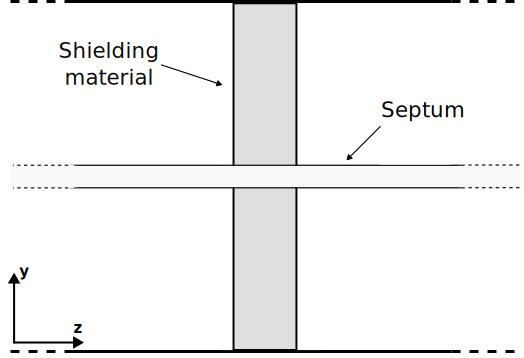
\includegraphics[width=\textwidth]{content//10_theory//img/ASTM ES7-83.png}
        \caption{Shielding material in TEM cell}
        \label{fig:ASTM ES7-83}
    \end{subfigure}%
    \hfill
    \begin{subfigure}[h]{0.49\textwidth}
        \centering
        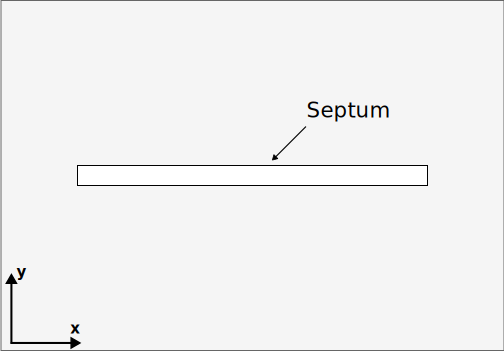
\includegraphics[width=\textwidth]{content//10_theory/img/form_of_shielding_material.png}
        \caption{Shape of the shielding material}
        \label{fig:form_of_shielding_material}
    \end{subfigure}
    \label{fig:subfigures}
\end{figure}

Then, the S-parameters derived in the simulations are used to get to the output powers $P_\mathrm{ref}$ and $P_\mathrm{load}$. By exciting the TEM cell with a power of 1\,W, the reference power $P_\mathrm{ref}=1\,\mathrm{W}$. The measured power is then derived through \autoref{eqn:load_power}.

\begin{equation}
    P_\mathrm{load}=P_\mathrm{ref}\cdot10^{|S_\mathrm{12}|/10}
    \label{eqn:load_power}
\end{equation}


\todo{Describe Method. Then follows dual TEM cells}

\subsubsection{Dual TEM cell}

The shielding effectiveness of a material may also be determined using two TEM cells, which are stacked upon each other, as shown in \autoref{fig:dual_tem_cell}. They are connected through an aperture, which can be filled with the shielding material. One TEM cell is excited, and therefore acts as a driving cell. It transmits power through the aperture. It is measured at the second TEM cell, which acts as a receiver. The dual TEM cell simulates near-field conditions, opposed to the far-field conditions simulated by the simple TEM cell \cite{MORARI_BĂLAN_2015}. This is important when using the shielding material to shield an antenna's radiation by placing the material directly next to it.

The electrically small aperture may be described by an electric and a magnetic dipole moment\todo{must it be electrically small?}. Their magnitude is related to the electric and magnetic coupling between the TEM cells over the aperture. Therefore, the electric and magnetic coupling can be determined separately by adding or subtracting the output powers of the receiving TEM cell \cite{MORARI_BĂLAN_2015, 4091811}. Consequently, a electric shielding effectiveness $SE_\mathrm{dB}^\mathrm{e}$ can be calculated with \autoref{eqn:se_dual_cell_e}, and a magnetic shielding effectiveness $SE_\mathrm{dB}^\mathrm{m}$ with \autoref{eqn:se_dual_cell_m}. If a material, for example, permits energy transfer because of magnetic dipoles in it, then a measurement with lower $SE_\mathrm{dB}^\mathrm{m}$ than $SE_\mathrm{dB}^\mathrm{e}$ is to be expected \cite{4091811}.


\begin{subequations}
    \begin{equation}
        SE_\mathrm{dB}^\mathrm{e}=10\log{\left( \frac{P_\mathrm{ref, sum}}{P_\mathrm{load,sum}} \right)}
        \label{eqn:se_dual_cell_e}
    \end{equation}
    \begin{equation}
        SE_\mathrm{dB}^\mathrm{m}=10\log{\left( \frac{P_\mathrm{ref, diff}}{P_\mathrm{load,diff}} \right)}
        \label{eqn:se_dual_cell_m}
    \end{equation}
\end{subequations}

Because the normalized electric field at the aperture will be of TEM mode, only the component normal to the aperture in z-direction has to be considered. Just as in the case of dipole representation, the Lorentz Reciprocity theorem may be applied to find the fields in the TEM cell. Because both the fields at the output and in the aperture are of TEM mode, only the E-field at the output may be considered. 

Since the aperture is electrically small, the field quantities may be assumed to be constant over it. This makes it possible to represent the energy transfer by dipole moments. \todo{Polarization of the material. Small aperture theory.}

\begin{figure}[h]
    \centering
    \includegraphics[width=0.75\linewidth]{content//10_theory//img/dual_tem_cell.png}
    \caption{Dual TEM cell with aperture}
    \label{fig:dual_tem_cell}
\end{figure}


\subsection{Radiated Field}

%
\subsection{Antenna Terminology}
Is this chapter necessary?
\subsection{Field regions}
Field regions, energy storage in each region, field distribution and auxiliary functions.

The region around an antenna may be divided into three sub-regions:
\begin{itemize}
	\item Reactive near-field region
	\item Radiating near-field or Fresnel region
	\item Far-field or Fraunhofer region
\end{itemize}

They are shown in \autoref{fig:fieldregionsantenna}. These regions are distinguished for most antennas using the wavelength $\lambda$ and the largest dimension of the antenna $D$. The nearest region to the antenna, the reactive near-field region, is a sphere with radius $R_1$, which is calculated with \autoref{eqn:region_r1}. It is characterized by the predominantly reactive fields in it. The next region, the radiating near-field region, is located around the first, within a sphere of radius $R_2$ calculated in \autoref{eqn:region_r2}. In there, the radiating fields dominate and the angular field distribution is dependent on the distance to the antenna. In the largest and last region, the far-field region, the angular field distribution is independent of the distance to the antenna \cite{Balanis_1997}.

\begin{subequations}
	\begin{equation}
		R_1=0.62\sqrt{D^3/\lambda}
		\label{eqn:region_r1}
	\end{equation}
	\begin{equation}
	R_2=2D^2/\lambda
	\label{eqn:region_r2}
	\end{equation}
\end{subequations}

\begin{figure}[h]
	\centering
	\includegraphics[width=0.7\linewidth]{content/10_theory/img/field_regions_antenna}
	\caption{Field regions of an antenna \cite{Balanis_1997}}
	\label{fig:fieldregionsantenna}
\end{figure}

The electrically short antennas located in the TEM cell interact with it mostly through the reactive near-field region. However, if the TEM cell is large and frequencies are high, the coupling occurs over the radiating near-field. There, the field distributions are different, hence the dipole moments couple differently over frequency to the cell. \todo[inline]{Is this even possible without reaching other modes behavior? And demonstrate the fields over frequency and distance, which changes differently in different regions}.



\subsection{Radiated Power}
Important for the Lorentz Reciprocity Part.



\section{Antennas}
\subsection{Antennas to Investigate}

% List possible electrically short antennas to investigate with dipole moments here. Describe, why they are interesting.


\section{Simulations}\label{sec:simulations}
\input{content/30_simulations/31_antennas}
\subsection{Dipole Moments}

\subsubsection{Orientation and position in TEM Cell}

\subsubsection{Combining dipole moments with antennas}



\input{content/30_simulations/33_shielding}
\FloatBarrier

\subsection{Investigation of field regions}

\todo[inline]{Update field plots}

In this section, the influence of the field region described in \autoref{sec:rad_fields} on the dipole moments are investigated. Making the TEM cell larger, such that $k\cdot r > 1$, is hardly possible without enabling higher-order modes to propagate. On the other hand, making the TEM cell smaller such that $k\cdot r \ll 1$, proves to be feasible. The following simulations are conducted with a TEM cell of dimensions $a=10\,\mathrm{mm}$ and $b=6\,\mathrm{mm}$, visible in \autoref{fig:krtemcell}.  

\begin{figure}[h]
	\centering
	\includegraphics[width=0.7\linewidth]{content/img/kr_tem_cell}
	\caption{TEM cell containing dipole moments}
	\label{fig:krtemcell}
\end{figure}


First, the current loop antenna used in \autoref{sec:loop_sim} is placed in the dead center of the TEM cell. The equivalent dipole moments are shown in \autoref{fig:loop_small_tem_moments}. In the \autoref{fig:dipole_moments_loop_antenna_copy} next to it, the dipole moments of the same antenna in the larger TEM cell used before ($a=40\,\mathrm{mm}$ and $b=24\,\mathrm{mm}$) are presented. 

\todo{The e field approx. in the python code is based on the large TEM cell. Therefore, the magnitude of the dipole moments of the small TEM cell are probably off}
\begin{figure}[htbp]
	\centering
	\begin{minipage}[t]{0.48\textwidth}
	\centering
\includegraphics[width=1\linewidth]{content/img/loop_small_tem_moments.png}
\caption{Moments in small TEM cell}
\label{fig:loop_small_tem_moments}
	\end{minipage}
	\hfill
	\begin{minipage}[t]{0.48\textwidth}
	\centering
	\includegraphics[width=1\linewidth]{content/img/dipole_moments_loop_antenna.png}
	\caption{Moments in normal TEM cell}
	\label{fig:dipole_moments_loop_antenna_copy}
	\end{minipage}
\end{figure}

This is done to compare the dipole moments in both cases. While they clearly increased by magnitude in case of the small TEM cell due to better coupling, their non-linear frequency relation still remains. This means that the change of field regions is not the reason for this behavior.

\todo{Insert kr, describe where r is measured, describe why the suspicion was that kr could influence this and how the fields change in the regions as described in the theoretical parts. Insert small current loop simulation. Insert Dipole Moment Simulations}

The $k\cdot r$ factor is determined in \autoref{fig:kranalysissmalltem} in the frequency range from 1\,MHz to 3\,GHz for the small TEM cell. This factor does not surpass 0.1, thus fulfilling the requirement $k\cdot r \ll 1$ for this investigation. For comparison, the $k\cdot r$ factor over a wider frequency range are shown in \autoref{fig:kranalysissmalltem} for the normal sized TEM cell ($a = 40\,\mathrm{mm}$ and $b = 24\,\mathrm{mm}$) and a degenerately high TEM cell ($a = 10\,\mathrm{mm}$ and $b=44\,\mathrm{mm}$). The high TEM does not have a port impedance of $50\,\Omega$, and is an attempt to achieve a large $k\cdot r$ factor without higher-order modes propagating. The markers in \autoref{fig:kranalysis} indicate the cut-off frequency, in which the next higher-order mode propagates. They demonstrate, that even in the high TEM cell a $k\cdot r = 1$ is not achieved.


\begin{figure}[htbp]
	\centering
	\begin{minipage}[t]{0.48\textwidth}
	\centering
	\includegraphics[width=1\linewidth]{content/img/kr_analysis_small_TEM}
	\caption{$k\cdot r$ in small TEM cell}
	\label{fig:kranalysissmalltem}
	\end{minipage}
	\hfill
	\begin{minipage}[t]{0.48\textwidth}
	\centering
	\includegraphics[width=1\linewidth]{content/img/kr_analysis}
	\caption{$k\cdot r$ for other TEM cells}
	\label{fig:kranalysis}
	\end{minipage}
\end{figure}
\todo{Fix figures: Titles and Legends}

Now, three simulations are conducted with different excitation sources in the small TEM cell:

\begin{itemize}
	\item The current loop 
	\item The equivalent dipole sources $e_z$ and $m_m$ of the current loop
	\item The equivalent magnetic dipole source $m_m$, neglecting $e_z$
\end{itemize}

\autoref{fig:outputpowercomparisonsmalltem} shows the output power over frequency normalized to 1\,W for all three constellations. The normalization is done to qualitatively discuss the frequency-dependent coupling behavior. \autoref{fig:phaseshiftcomparisonsmalltem} demonstrates the phase shift between the powers at the two waveports over frequency.

\begin{figure}[htbp]
	\centering
	\begin{minipage}[t]{0.48\textwidth}
		\centering
		\includegraphics[width=1\linewidth]{content/img/output_power_comparison_small_tem}
		\caption{Output powers}
		\label{fig:outputpowercomparisonsmalltem}
	\end{minipage}
	\hfill
	\begin{minipage}[t]{0.48\textwidth}
		\centering
		\includegraphics[width=1\linewidth]{content/img/phase_shift_comparison_small_tem}
		\caption{Phase shifts}
		\label{fig:phaseshiftcomparisonsmalltem}
	\end{minipage}
\end{figure}

The frequency dependent behavior of the output power does not change depending on the type of dipole moment used. This is significant, because this shows that the dipole moments do not exhibit different coupling behaviors in the TEM cells. This is further proven in the phase shift plots. The magnetic dipole moment causes a constant phase shift of $-\pi$. If this was not the case, this would mean that the coupling behavior of the magnetic dipole moment in the TEM cell would change. Since the opposite is the case, this poses as good evidence against arguments of change in field regions causing the non-linear dipole moment behavior. Instead, it is very likely to be caused by the geometry of the antenna.



\todo{Const antenna power definieren, damit dipolmomente einzelner antennen vergleichbar wird}


\newpage

\iffalse
\subsection{Summary}

\fi
\cleardoublepage
\printbibliography
\end{document}
